\section{Empirical Results}

Our experiments are designed to answer the research questions presented in Section \ref{sec:introduction}. We answer RQ1 (can we frame document selection as a multi-armed bandit problem?) through experiments on NeuCLIR and ResearchyQuestions in Section \ref{section:neuclir_eval}. We answer RQ2 (do policy-observed documents lead to better performance on downstream tasks?) by long-form generation of reports on NeuCLIR in Section \ref{section:neuclir_downstream_task}. We answer RQ3 (can we apply bandit-learning on hierarchical sub-queries?) by modeling correlated bandits on existing sub-query splits from ResearchyQuestions in Section \ref{section:researchy_correlated}. 


\subsection{Document selection as a multi-armed bandit problem}\label{section:neuclir_eval}

% \begin{table*}[!ht]
%   \centering
%   {\small
%   \setlength{\tabcolsep}{5pt}      % horizontal padding
%   \renewcommand{\arraystretch}{1.2} % row height
%   \begin{tabular}{l*{5}{c}}
%     \toprule
%     & \makecell{Citation\\Relevance\\Macro} 
%     & \makecell{Citation\\Support\\Macro} 
%     & \makecell{Nugget\\Coverage\\Macro} 
%     & \makecell{Sentence\\Support\\Macro} 
%     & \makecell{F\textsubscript{1}\\Macro} \\
%     \midrule
%     Random               & 1.0 & $0.8257 \pm 0.043$ & $0.4767 \pm 0.055$ & $0.8216 \pm 0.045$ & $0.5885 \pm 0.048$ \\
%     Rank                 & 1.0 & $0.8343 \pm 0.038$ & $0.4621 \pm 0.045$ & $0.8189 \pm 0.045$ & $0.5732 \pm 0.040$ \\
%     \midrule
%     $\epsilon$-greedy    & 1.0 & $0.8226 \pm 0.042$ & $0.4896 \pm 0.053$ & $0.8090 \pm 0.049$ & $0.5968 \pm 0.043$ \\
% %    Bernoulli            & -&	-&	-&	-&	- \\
%     Bernoulli UCB        & 1.0 & $0.8343 \pm 0.031$ & $0.4767 \pm 0.042$ & $0.8232 \pm 0.037$ & $0.5883 \pm 0.037$ \\
% %    Bernoulli $k=3$      & 0.8795 & 0.8284 & 0.4479 & 0.8212 & 0.5555 \\
%     Bernoulli $k=4$      & 1.0 & $\textbf{0.8656} \pm \textbf{0.037}$ & $0.4625 \pm 0.044$ & $\textbf{0.8552} \pm \textbf{0.039}$ & $0.5831 \pm 0.039$ \\
%     Bernoulli $k=5$      & 1.0 & $0.8491 \pm 0.035$ & $\textbf{0.4923} \pm \textbf{0.045}$ & $0.8385 \pm 0.038$ & $\textbf{0.6035} \pm \textbf{0.038}$ \\
% %    Bernoulli Rank-aware & 0.8629 &	0.7882 & 0.4611 & 0.7798 & 0.5556 \\
% %    Gaussian             & 0.8177 & 0.7916 & 0.4117 & 0.7941 & 0.5270 \\
% %    Gaussian ING         & 0.8118 & 0.8057 & 0.4291 & 0.8037 & 0.5470 \\
% %    Diversity            & 0.8629 &	0.7864 & 0.4611 & 0.7788 & 0.5566 \\
% %    Diversity Concave    & 0.8522 &	0.7962 & 0.4367 & 0.7965 & 0.5507 \\
%     Top-K UCB Diversity  & 1.0 & $0.8369 \pm 0.031$ & $0.4626 \pm 0.040$ & $0.8357 \pm 0.030$ & $0.5798 \pm 0.036$ \\
%     \bottomrule
%   \end{tabular}
%   }
%   \caption{Report Generation results for budget \(b = 20\%\).}
%   \label{tab:neuclir_report_generation_b20}
% \end{table*}


% \begin{table*}[t!]
%   \centering
%   {\small
%   \setlength{\tabcolsep}{5pt}      % horizontal padding
%   \renewcommand{\arraystretch}{1.2} % row height
%   \begin{tabular}{l*{5}{c}}
%     \toprule
%     & \makecell{Citation\\Relevance\\Macro} 
%     & \makecell{Citation\\Support\\Macro} 
%     & \makecell{Nugget\\Coverage\\Macro} 
%     & \makecell{Sentence\\Support\\Macro} 
%     & \makecell{F\textsubscript{1}\\Macro} \\
%     \midrule
%     Full   & 0.8629	& 0.7882 & 0.4611 &	0.7798 & 0.5556 \\
%     \midrule
%     Random               & 1.0 & $0.8272 \pm 0.054$ & $0.4463 \pm 0.052$ & $\textbf{0.8368} \pm \textbf{0.055}$ & $0.5658 \pm 0.480$ \\
%     Rank                 & 1.0 & $0.8184 \pm 0.053$ & $0.4622 \pm 0.06$ & $0.7909 \pm 0.067$ & $0.5661 \pm 0.061$ \\
%     \midrule
%     $\epsilon$-greedy    & 1.0 & $0.7994 \pm 0.071$ & $0.4777 \pm 0.080$ & $0.7745 \pm 0.077$ & $0.5716 \pm 0.065$ \\
% %    Bernoulli            & -&	-&	-&	-&	- \\
%     Bernoulli UCB        & 1.0 & $0.8299 \pm 0.051$ & $0.4967 \pm 0.071$ & $0.7978 \pm 0.080$ & $0.5727 \pm 0.070$ \\
% %    Bernoulli $k=3$      & 0.8795 & 0.8284 & 0.4479 & 0.8212 & 0.5555 \\
%     Bernoulli $k=4$      & 1.0 & $0.8340 \pm 0.060$ & $0.4804 \pm 0.075$ & $0.8171 \pm 0.075$ & $0.5796 \pm 0.064$ \\
%     Bernoulli $k=5$      & 1.0 & $0.8313 \pm 0.056$ & $\textbf{0.5002} \pm \textbf{0.064}$ & $0.8193 \pm 0.072$ & $\textbf{0.5994} \pm \textbf{0.060}$ \\
% %    Bernoulli Rank-aware & 0.8629 &	0.7882 & 0.4611 & 0.7798 & 0.5556 \\
% %    Gaussian             & 0.8177 & 0.7916 & 0.4117 & 0.7941 & 0.5270 \\
% %    Gaussian ING         & 0.8118 & 0.8057 & 0.4291 & 0.8037 & 0.5470 \\
% %    Diversity            & 0.8629 &	0.7864 & 0.4611 & 0.7788 & 0.5566 \\
% %    Diversity Concave    & 0.8522 &	0.7962 & 0.4367 & 0.7965 & 0.5507 \\
%     Top-K UCB Diversity  & 1.0 & $\textbf{0.8346} \pm \textbf{0.046}$ & $0.4747 \pm 0.050$ & $0.8260 \pm 0.0610$ & $0.5809 \pm 0.060$ \\
%     \bottomrule
%   \end{tabular}
%   }
%   \caption{Report Generation results for budget \(b = 30\%\).}
%   \label{tab:neuclir_report_generation_b30}
% \end{table*}


% \begin{table*}[!ht]
%   \centering
%   {\small
%   \setlength{\tabcolsep}{5pt}      % horizontal padding
%   \renewcommand{\arraystretch}{1.2} % row height
%   \begin{tabular}{l*{4}{c}}
%     \toprule
%     & \makecell{Citation\\Support\\Macro} 
%     & \makecell{Nugget\\Coverage\\Macro} 
%     & \makecell{Sentence\\Support\\Macro} 
%     & \makecell{F\textsubscript{1}\\Macro} \\
%     \midrule
%     Full   & 0.7882 & 0.4611 &	0.7798 & 0.5556 \\
%     \midrule
%     Random               & $0.8257 \pm 0.043$ & $0.4767 \pm 0.055$ & $0.8216 \pm 0.045$ & $0.5885 \pm 0.048$ \\
%     Rank                 & $0.8343 \pm 0.038$ & $0.4621 \pm 0.045$ & $0.8189 \pm 0.045$ & $0.5732 \pm 0.040$ \\
%     \midrule
%     $\epsilon$-greedy    & $0.8226 \pm 0.042$ & $0.4896 \pm 0.053$ & $0.8090 \pm 0.049$ & $0.5968 \pm 0.043$ \\
% %    Bernoulli            & -&	-&	-&	-&	- \\
%     Bernoulli UCB        & $0.8343 \pm 0.031$ & $0.4767 \pm 0.042$ & $0.8232 \pm 0.037$ & $0.5883 \pm 0.037$ \\
% %    Bernoulli $k=3$      & 0.8795 & 0.8284 & 0.4479 & 0.8212 & 0.5555 \\
%     Bernoulli $k=4$      & $\textbf{0.8656} \pm \textbf{0.037}$ & $0.4625 \pm 0.044$ & $\textbf{0.8552} \pm \textbf{0.039}$ & $0.5831 \pm 0.039$ \\
%     Bernoulli $k=5$      & $0.8491 \pm 0.035$ & $\textbf{0.4923} \pm \textbf{0.045}$ & $0.8385 \pm 0.038$ & $\textbf{0.6035} \pm \textbf{0.038}$ \\
% %    Bernoulli Rank-aware & 0.8629 &	0.7882 & 0.4611 & 0.7798 & 0.5556 \\
% %    Gaussian             & 0.8177 & 0.7916 & 0.4117 & 0.7941 & 0.5270 \\
% %    Gaussian ING         & 0.8118 & 0.8057 & 0.4291 & 0.8037 & 0.5470 \\
% %    Diversity            & 0.8629 &	0.7864 & 0.4611 & 0.7788 & 0.5566 \\
% %    Diversity Concave    & 0.8522 &	0.7962 & 0.4367 & 0.7965 & 0.5507 \\
%     Top-K UCB Diversity  & $0.8369 \pm 0.031$ & $0.4626 \pm 0.040$ & $0.8357 \pm 0.030$ & $0.5798 \pm 0.036$ \\
%     \bottomrule
%   \end{tabular}
%   }
%   \caption{Report Generation results for budget \(b = 20\%\).}
%   \label{tab:neuclir_report_generation_b20}
% \end{table*}


% \begin{table*}[t!]
%   \centering
%   {\small
%   \setlength{\tabcolsep}{5pt}      % horizontal padding
%   \renewcommand{\arraystretch}{1.2} % row height
%   \begin{tabular}{l*{4}{c}}
%     \toprule
%     & \makecell{Citation\\Support\\Macro} 
%     & \makecell{Nugget\\Coverage\\Macro} 
%     & \makecell{Sentence\\Support\\Macro} 
%     & \makecell{F\textsubscript{1}\\Macro} \\
%     \midrule
%     Full   & 0.7882 & 0.4611 &	0.7798 & 0.5556 \\
%     \midrule
%     Random               & $0.8272 \pm 0.054$ & $0.4463 \pm 0.052$ & $\textbf{0.8368} \pm \textbf{0.055}$ & $0.5658 \pm 0.480$ \\
%     Rank                 & $0.8184 \pm 0.053$ & $0.4622 \pm 0.06$ & $0.7909 \pm 0.067$ & $0.5661 \pm 0.061$ \\
%     \midrule
%     $\epsilon$-greedy    & $0.7994 \pm 0.071$ & $0.4777 \pm 0.080$ & $0.7745 \pm 0.077$ & $0.5716 \pm 0.065$ \\
% %    Bernoulli            & -&	-&	-&	-&	- \\
%     Bernoulli UCB        & $0.8299 \pm 0.051$ & $0.4967 \pm 0.071$ & $0.7978 \pm 0.080$ & $0.5727 \pm 0.070$ \\
% %    Bernoulli $k=3$      & 0.8795 & 0.8284 & 0.4479 & 0.8212 & 0.5555 \\
%     Bernoulli $k=4$      & $0.8340 \pm 0.060$ & $0.4804 \pm 0.075$ & $0.8171 \pm 0.075$ & $0.5796 \pm 0.064$ \\
%     Bernoulli $k=5$      & $0.8313 \pm 0.056$ & $\textbf{0.5002} \pm \textbf{0.064}$ & $0.8193 \pm 0.072$ & $\textbf{0.5994} \pm \textbf{0.060}$ \\
% %    Bernoulli Rank-aware & 0.8629 &	0.7882 & 0.4611 & 0.7798 & 0.5556 \\
% %    Gaussian             & 0.8177 & 0.7916 & 0.4117 & 0.7941 & 0.5270 \\
% %    Gaussian ING         & 0.8118 & 0.8057 & 0.4291 & 0.8037 & 0.5470 \\
% %    Diversity            & 0.8629 &	0.7864 & 0.4611 & 0.7788 & 0.5566 \\
% %    Diversity Concave    & 0.8522 &	0.7962 & 0.4367 & 0.7965 & 0.5507 \\
%     Top-K UCB Diversity  & $\textbf{0.8346} \pm \textbf{0.046}$ & $0.4747 \pm 0.050$ & $0.8260 \pm 0.0610$ & $0.5809 \pm 0.060$ \\
%     \bottomrule
%   \end{tabular}
%   }
%   \caption{Report Generation results for budget \(b = 30\%\).}
%   \label{tab:neuclir_report_generation_b30}
% \end{table*}

\begin{table*}[!ht]
  \centering
  \setlength{\tabcolsep}{5pt}      % horizontal padding
  \renewcommand{\arraystretch}{1.2} % row height
  \resizebox{\linewidth}{!}{%
  \begin{tabular}{l*{6}{c}}
    \toprule
    & \multicolumn{3}{c}{Budget $b=20\%$} & \multicolumn{3}{c}{Budget $b=30\%$} \\
    \cmidrule(lr){2-4} \cmidrule(lr){5-7}
    & \makecell{Citation\\Support} 
    & \makecell{Nugget\\Coverage} 
    & \makecell{Sentence\\Support} 
    & \makecell{Citation\\Support} 
    & \makecell{Nugget\\Coverage} 
    & \makecell{Sentence\\Support} \\
    \midrule
    Full   & 0.788 & 0.461 & 0.780 & 0.788 & 0.461 & 0.780 \\
    \midrule
    Random               & $0.826 \pm 0.043$ & $0.477 \pm 0.055$ & $0.822 \pm 0.045$ & $0.827 \pm 0.054$ & $0.446 \pm 0.052$ & $\textbf{0.837} \pm \textbf{0.055}$ \\
    Rank                 & $0.834 \pm 0.038$ & $0.462 \pm 0.045$ & $0.819 \pm 0.045$ & $0.818 \pm 0.053$ & $0.462 \pm 0.060$ & $0.791 \pm 0.067$ \\
    \midrule
    $\epsilon$-greedy    & $0.823 \pm 0.042$ & $0.490 \pm 0.053$ & $0.809 \pm 0.049$ & $0.799 \pm 0.071$ & $0.478 \pm 0.080$ & $0.775 \pm 0.077$ \\
    Bernoulli UCB        & $0.834 \pm 0.031$ & $0.477 \pm 0.042$ & $0.823 \pm 0.037$ & $0.830 \pm 0.051$ & $0.497 \pm 0.071$ & $0.798 \pm 0.080$ \\
    Bernoulli $k=4$      & $\textbf{0.866} \pm \textbf{0.037}$ & $0.463 \pm 0.044$ & $\textbf{0.855} \pm \textbf{0.039}$ & $0.834 \pm 0.060$ & $0.480 \pm 0.075$ & $0.817 \pm 0.075$ \\
    Bernoulli $k=5$      & $0.849 \pm 0.035$ & $\textbf{0.492} \pm \textbf{0.045}$ & $0.839 \pm 0.038$ & $0.831 \pm 0.056$ & $\textbf{0.500} \pm \textbf{0.064}$ & $0.819 \pm 0.072$ \\
    Top-K UCB Div.  & $0.837 \pm 0.031$ & $0.463 \pm 0.040$ & $0.836 \pm 0.030$ & $\textbf{0.835} \pm \textbf{0.046}$ & $0.475 \pm 0.050$ & $0.826 \pm 0.061$ \\
    \bottomrule
  \end{tabular}
  }
  \caption{Report Generation results for budgets \(b=20\%\) and \(b=30\%\) with their confidence intervals. Selecting a relevant subset of documents boosts downstream report generation performance with \(6.0\)--\(9.9\%\) increase in citation support, \(6.7\)--\(8.5\%\) in nugget coverage, and \(7.3\)--\(9.6\%\) in sentence support.}
  \label{tab:neuclir_report_generation_b20_b30}
\end{table*}




Figure \ref{fig:neuclir_precision} illustrates macro-precision over document budget. We highlight the main findings in Figure \ref{fig:neuclir_precision}, while Figures \ref{fig:neuclir_precision_all} and \ref{fig:researchy_eval_all} in the Appendix present all results. Exploitation and exploration-only policies perform similarly to our baselines: the exploitation-only policy returns a precision of \(0.57\) and exploration-only a precision of \(0.55\) on NeuCLIR, while both exploitation and exploitation-only achieve \(0.14\) precision on ResearchyQuestions. Based on results on our proposed rewards, we observe that: (i) reward policies effectively model sub-query relevance; (ii) \(\epsilon\text{-greedy}\) performs best when using \(10\)--\(20\%\) of the budget, likely because early exploitation of high-relevance arms is optimal; and (iii) using rank-information gives a noticeable advantage. All rewards achieve the same macro-precision as the budget reaches maximum value, due to coverage of the same set of documents by all policies and baselines. Figure \ref{fig:neuclir_recall_all} (in the Appendix) shows similar insights on recall w.r.t.\ the total amount of relevant documents retrieved for all sub-queries.


\begin{table}[ht]
  \centering
  \setlength{\tabcolsep}{3.5pt}
  \renewcommand{\arraystretch}{1.2}
  \resizebox{\linewidth}{!}{%
  \begin{tabular}{l*{5}{c}*{2}{c}}
    \toprule
     & \multicolumn{5}{c}{\makecell{\textbf{\(\alpha\text{-nDCG}\)} $\uparrow$ \\ NeuCLIR24}} 
     & \multicolumn{2}{c}{\makecell{\textbf{\(\alpha\text{-nDCG}\)} $\uparrow$ \\ Researchy}} \\
    \cmidrule(lr){2-6} \cmidrule(lr){7-8}
     & $K{=}5$ & $K{=}10$ & $K{=}20$ & $K{=}40$ & $K{=}50$ & $K{=}5$ & $K{=}10$ \\
    \midrule
    Random               & 0.411 & 0.454 & 0.479 & 0.263 & 0.311 & 0.134 & 0.127 \\
    Rank                 & 0.426 & 0.462 & 0.476 & 0.265 & \underline{0.313} & 0.172 & 0.137 \\
    \midrule
    $\epsilon$-greedy    & \textbf{0.500} & \textbf{0.539} & 0.546 & \textbf{0.286} & \textbf{0.314} & 0.207 & 0.145 \\
    Bernoulli            & 0.445 & 0.508 & 0.543 & 0.246 & 0.282 & 0.210 & \underline{0.157} \\
    Bernoulli UCB        & 0.460 & 0.517 & 0.545 & 0.248 & 0.279 & 0.210 & \textbf{0.164} \\
%    Bernoulli $k=3$      & 0.462 & 0.531 & \textbf{0.556} & 0.264 & 0.285 & 0.230 & 0.155 \\
    Bernoulli $k=4$      & 0.461 & 0.536 & 0.551 & \underline{0.275} & 0.283 & \textbf{0.240} & 0.153 \\
    Bernoulli $k=5$      & 0.448 & 0.523 & \textbf{0.555} & 0.267 & 0.291 & \underline{0.232} & 0.156 \\
    Bernoulli Rank       & 0.437 & 0.481 & 0.523 & 0.264 & 0.289 & 0.208 & 0.156 \\
%    Gaussian             & 0.413 & 0.442 & 0.468 & 0.252 & 0.281 & 0.172 & 0.140 \\
%    Gaussian ING         & 0.409 & 0.445 & 0.463 & 0.259 & 0.284 & 0.170 & 0.135 \\
    Diversity            & 0.444 & 0.505 & 0.541 & 0.260 & 0.281 & 0.210 & 0.154 \\
    Diversity Conc.      & 0.442 & 0.512 & 0.540 & 0.260 & 0.283 & 0.211 & 0.149 \\
    Top-$k$ UCB Div.  & \underline{0.469} & \underline{0.537} & \underline{0.552} & 0.253 & 0.285 & 0.222 & 0.154 \\
    \bottomrule
  \end{tabular}
  }
  \caption{Comparison of $\alpha$-nDCG over different budgets \(k\) for NeuCLIR24 and ResearcyQuestions. Bernoulli posteriors are the best to estimate document relevance regardless the value of \(k\) for $\alpha$-nDCG, with an additional performance boost when considering the top k ranked documents. UCB also brings an advantage. Div. in the last metrics refers to Diversity.}
  \label{tab:neuclir_alphandcg}
\end{table}


%Figures \ref{fig:researchy_eval} and \ref{fig:researchy_eval_all} presents the macro-precision results across all budgets on ResearchyQuestions, presented as percentages. Unlike NeuCLIR, ResearchyQuestions has a fixed set of generated sub-queries, and the number varies per instance. The figure expressed our main findings, which are in line with the previously seen trend in NeuCLIR: (1) reward-based policies outperform the baselines in most settings, except for the continuous policies; (2) we notice a high performance for all Bernoulli based policies from the beginning, with a noticeable increase for budgets \(b \in [10\%, 20\%]\); (3) using ranked-list positions in top-k policies rings a boost in performance, and (4) incorporating diversity does not necessarily add to performance.



Table \ref{tab:neuclir_alphandcg} shows results for multiple values of \(\alpha\text{-nDCG}\). We observe that \(\alpha\text{-nDCG}\) achieves higher values for baselines and all policies for budget \(K \in [5, 10, 20]\). As the budget grows, all baselines and policies converge towards the same pool of documents, reducing marginal novelty, as \(\alpha\text{-nDCG}\) punishes redundant content. Out of all policies, notably the \(\epsilon\text{-greedy}\), UCB, and ranked Bernoulli rewards perform the best. %We also notice a decline in \(\alpha\text{-nDCG}\) as the budget increases, with baselines becoming better, one reason being that the document diversity converges between policies as the sampling set is reduced.

We frame query decomposition and document selection as a stochastic multi-armed bandit where each subquery is an independent arm, and pulling an arm corresponds to observing a document down the ranked list. Each observation receives a Bernoulli reward based on relevance, updating the subquery’s relevance distribution. Across experiments, we show that bandit learning outperforms full exploitation and exploration, and that a policy combining rank-information, diversity, and an upper confidence bound (Equation \ref{eq:top_reward}) outperforms other variants in Table \ref{tab:reward_functions}.




\subsection{Impact on report generation}\label{section:neuclir_downstream_task}

% We use document subsets found by our policies for budgets \(b=[20\%;30\%]\) for report generation on NeuCLIR24. We select these budgets as they showed the best trade-off between evidence coverage in preliminary experiments (see Figure \ref{fig:neuclir_precision}). We evaluate the generations using the Auto-ARGUE framework that computes 4 metrics, i.e., citation relevance (how well cited documents are), citation support (assesses whether the citations support the documents), nugget coverage (proportion of unique nuggets), and sentence support (proportion of sentences needing citation support). An example of a generated report is shown in Appendix \ref{sec:app_report_gen_example}. The results in Table \ref{tab:neuclir_report_generation_b20_b30} show that top-$k$ Bernoulli policies perform best in both covering relevant nuggets and supporting facts with citations. We do not report citation relevance when selecting relevant documents, as the metric remains constant between policies.

We generate reports on NeuCLIR24 using document subsets retrieved by our policies for budgets \(b=[20\%;30\%]\), which provided the best trade-off between evidence coverage and precision in preliminary experiments (Figure~\ref{fig:neuclir_precision}). Evaluations are conducted with the Auto-ARGUE framework, which measures four aspects of grounded generation: citation relevance (quality of cited sources), citation support (alignment between claims and citations), nugget coverage (proportion of unique information units), and sentence support (share of sentences with appropriate evidence).
An example report is provided in Appendix~\ref{sec:app_report_gen_example}.
As shown in Table~\ref{tab:neuclir_report_generation_b20_b30}, top-$k$ Bernoulli policies achieve the strongest performance in both nugget coverage and factual support. Citation relevance is omitted, as it remains constant across policies. Results show that selecting documents using multi-armed bandits improves downstream report generation. The strongest performance gains follow the rank-aware top-$k$ Bernoulli policies, including top-$k$ UCB with diversity \emph{citation support} at $b{=}30\%$ ($0.835$). 


% \begin{table}[h]
%   \centering
%   {\scriptsize
%   \setlength{\tabcolsep}{3.5pt}
%   \renewcommand{\arraystretch}{1.2}
%   \begin{tabular}{l|*{5}{c}|*{2}{c}}
%     \toprule
%      & \multicolumn{5}{c|}{\makecell{\textbf{\(\alpha\text{-nDCG}\)} $\uparrow$ \\ NeuCLIR24}} 
%      & \multicolumn{2}{c}{\makecell{\textbf{\(\alpha\text{-nDCG}\)} $\uparrow$ \\ Researchy}} \\
%     \cmidrule(lr){2-6} \cmidrule(lr){7-8}
%      & k=5 & k=10 & k=20 & k=40 & k=50 & k=5 & k=10 \\
%     \midrule
%     Random               & 0.411 & 0.454 & 0.479 & 0.263 & 0.311 & 0.134 & 0.127 \\
%     Rank                 & 0.426 & 0.462 & 0.476 & 0.265 & \textbf{0.313} & 0.172 & 0.137 \\
%     \midrule
%     $\epsilon$-greedy    & \textbf{0.500} & \textbf{0.539} & 0.546 & \textbf{0.286} & \textbf{0.314} & 0.207 & 0.145 \\
%     Bernoulli            & 0.445 & 0.508 & 0.543 & 0.246 & 0.282 & 0.210 & \textbf{0.157} \\
%     Bernoulli UCB        & 0.460 & 0.517 & 0.545 & 0.248 & 0.279 & 0.210 & \textbf{0.164} \\
%     Bernoulli $k=3$      & \textbf{0.462} & 0.531 & \textbf{0.556} & 0.264 & 0.285 & \textbf{0.230} & 0.155 \\
%     Bernoulli $k=4$      & 0.461 & \textbf{0.536} & 0.551 & \textbf{0.275} & 0.283 & \textbf{0.240} & 0.153 \\
%     Bernoulli $k=5$      & 0.448 & 0.523 & \textbf{0.555} & \textbf{0.267} & \textbf{0.291} & \textbf{0.232} & \textbf{0.156} \\
%     Bernoulli Rank       & 0.437 & 0.481 & 0.523 & 0.264 & 0.289 & 0.208 & \textbf{0.156} \\
% %    Gaussian             & 0.413 & 0.442 & 0.468 & 0.252 & 0.281 & 0.172 & 0.140 \\
% %    Gaussian ING         & 0.409 & 0.445 & 0.463 & 0.259 & 0.284 & 0.170 & 0.135 \\
%     Diversity            & 0.444 & 0.505 & 0.541 & 0.260 & 0.281 & 0.210 & 0.154 \\
%     Diversity Conc.      & 0.442 & 0.512 & 0.540 & 0.260 & 0.283 & 0.211 & 0.149 \\
%     Top-K UCB Diversity  & \textbf{0.469} & \textbf{0.537} & \textbf{0.552} & 0.253 & 0.285 & 0.222 & 0.154 \\
%     \bottomrule
%   \end{tabular}
%   }
%   \caption{Comparison of $\alpha$-nDCG with different values of \(k\) over NeuCLIR24 and ResearcyQuestions. Bernoulli posteriors are the best to estimate document relevance regardless the value of \(k\) for $\alpha$-nDCG, with an additioanl performance boost when considering the top k ranked documents. UCB also brings an advantage.}
%   \label{tab:neuclir_alphandcg}
% \end{table}


\subsection{Bandit learning for hierarchical sub-queries}\label{section:researchy_correlated}

We use ResearchyQuestions to evaluate our correlated bandits formulation. Results in Table \ref{tab:budget10_results} show clear improvements over policies for a small budget \(b = 10\%\). 
%; given that ResearchyQuestions is a sparse dataset wrt. document relevance, as the budget increases, it is very likely that the first level of sub-queries is being explored and therefore values converge. For a full analysis and comparison, see Figure \ref{fig:researchy_correlated} in the Appendix. 
We pick the three hyperparameters described in Section \ref{sec:hierarchical_method} through Bayesian hyperparameter search. The results are presented in Figure \ref{fig:bayesian_lookup} in the Appendix, given which we chose a minimal number of observations \(n=4\), informativeness threshold \(\tau=0.77\), and inheritance factor \(\lambda=0.91\).

Table \ref{tab:budget10_results} shows that we can use bandit-learning to model hierarchical query decomposition. For budget \(b=10\%\), there is a clear performance boost when using the hierarchical structure compared to treating all subqueries at the same serial level. 
Performance using Bernoulli increases by \(21.6\%\), while top-\(k=5\) has a performance boost of \(32.3\%\), and RL top-\(k\) UCB diversity a gain of \(20.4\%\). As the budget increases, the gains converge. These results indicate that hierarchy-aware (correlated) bandits best balance exploration/exploitation early by focusing on promising branches of the sub-query tree, yielding higher precision under small budgets.




% \begin{table}[ht]
%   \centering
%   {\scriptsize
%   \setlength{\tabcolsep}{4.5pt}
%   \renewcommand{\arraystretch}{1.2}
%   \begin{tabular}{l|*{2}{c}|*{2}{c}}
%     \toprule
%      & \multicolumn{2}{c|}{\textbf{\(b = 10\%\)}} & \multicolumn{2}{c}{\textbf{\(b = 20\%\)}} \\
%     \cmidrule(lr){2-3} \cmidrule(lr){4-5}
%      & S. & H. & S. & H. \\
%     \midrule
%     Baseline Random              & 0.1570 & 0.1588 & 0.1374 & 0.1351 \\
%     Baseline Rank-aware          & 0.2635 & 0.2631 & 0.1914 & 0.1927 \\
%     $\epsilon$-greedy strategy   & 0.3061 & 0.3079 & 0.2225 & 0.2226 \\
%     Bernoulli                    & 0.3049 & \underline{0.3625} & 0.2372 & 0.2454 \\
%     Bernoulli UCB                & 0.3056 & \underline{0.3607} & 0.2342 & 0.2440 \\
%     Bernoulli Top k=3            & 0.3246 & \underline{0.3863} & 0.2604 & 0.2583 \\
%     Bernoulli Top k=4            & 0.3166 & \underline{0.3924} & 0.2608 & 0.2624 \\
%     Bernoulli Top k=5            & 0.3034 & \underline{0.3910} & 0.2571 & 0.2673 \\
%     Bernoulli Rank-Aware         & 0.3042 & \underline{0.3626} & 0.2324 & 0.2469 \\
%     Gaussian                     & 0.2600 & 0.2631 & 0.1997 & 0.1927 \\
%     Gaussian ING                 & 0.2644 & 0.2631 & 0.2011 & 0.1927 \\
%     Bernoulli Diversity          & 0.3050 & \underline{0.3621} & 0.2365 & 0.2445 \\
%     Bernoulli Diversity Concave  & 0.3063 & \underline{0.3618} & 0.2360 & 0.2450 \\
%     RL top k ucb diversity       & 0.3244 & \underline{0.3843} & 0.2560 & 0.2577 \\
%     \bottomrule
%   \end{tabular}
%   }
%   \caption{Comparison of precision under budgets \(b = 10\%\) and \(b=20\%\) for both serialized and hierarchical document selection strategies with correlated bandits. The \underline{underlined} values represent clear improvements.}
%   \label{tab:budget10_results}
% \end{table}


\begin{table}[ht]
  \centering
  \setlength{\tabcolsep}{4.5pt}
  \renewcommand{\arraystretch}{1.2}
  \resizebox{\linewidth}{!}{%
  \begin{tabular}{l *{2}{c} *{2}{c}}
    \toprule
     & \multicolumn{2}{c}{\textbf{\(b = 10\%\)}} & \multicolumn{2}{c}{\textbf{\(b = 20\%\)}} \\
    \cmidrule(lr){2-3} \cmidrule(lr){4-5}
     & Ser. & Hier. & Ser. & Hier. \\
    \midrule
    Baseline Random              & 0.157 & 0.159 & 0.137 & 0.136 \\
    Baseline Rank-aware          & 0.263 & 0.264 & 0.191 & 0.193 \\
    $\epsilon$-greedy strategy   & 0.306 & 0.306 & 0.223 & 0.223 \\
    Bernoulli                    & 0.305 & \textbf{0.371} & 0.237 & 0.246 \\
    Bernoulli UCB                & 0.306 & \textbf{0.368} & 0.234 & 0.245 \\
    Bernoulli Top $k=3$            & 0.325 & \textbf{0.391} & 0.260 & 0.250 \\
    Bernoulli Top $k=4$            & 0.317 & \textbf{0.398} & 0.261 & 0.2512 \\
    Bernoulli Top $k=5$            & 0.303 & \textbf{0.401} & 0.257 & 0.250 \\
    Bernoulli Rank-Aware         & 0.304 & \textbf{0.375} & 0.232 & 0.242 \\
    Gaussian                     & 0.260 & 0.264 & 0.200 & 0.197 \\
    Gaussian ING                 & 0.264 & 0.263 & 0.201 & 0.189 \\
    Bernoulli Diversity          & 0.305 & \textbf{0.371} & 0.237 & 0.247 \\
    Bernoulli Diversity Concave  & 0.306 & \textbf{0.371} & 0.236 & 0.247 \\
    RL Top-$k$ UCB diversity     & 0.324 & \textbf{0.390} & 0.256 & 0.249 \\
    \bottomrule
  \end{tabular}
  }
  \caption{Comparison of precision under budgets \(b = 10\%\) and \(b=20\%\) for both serialized (Ser.) and hierarchical (Hier.) document selection strategies with correlated bandits. For all discrete estimate policies, selecting a subset of documents by taking into account sub-query hierarchies yields better performance, with Bernoulli top \(k=5\) having a \(24\%\) performance boost over the serialized representation, where we use the number of observations \(n=4\), informativeness threshold \(\tau=0.77\) and inheritance factor \(\lambda=0.91\)}
  \label{tab:budget10_results}
\end{table}


\subsection{NeuCLIR analysis}\label{section:neuclir_analysis}

\header{Rank information} We run our experiments in a setting where each sub-query corresponds to a ranked list of documents. Therefore, we make the assumption that the ranked list is a good reflection of document relevance. To verify this hypothesis, we calculate the mean reciprocal rank and fit a linear regression to estimate whether the rank is negatively correlated with the relevance of the documents. Figure \ref{fig:slope_neuclir} shows that very few instances have a negative slope, indicating that the ranked lists are not always consistent with relevance.

\begin{figure}[ht]
    \centering
    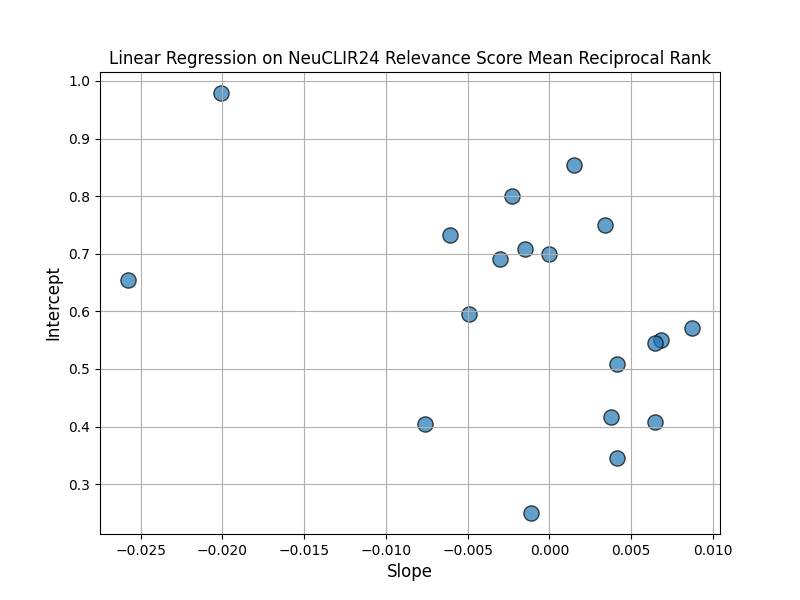
\includegraphics[clip,trim=12mm 4mm 12mm 12mm, width=\linewidth]{images/relevance_test_scatterplot.png}
    \caption{Fitting linear regression functions \(y = \alpha + \beta x +\epsilon\) between the mean reciprocal ranks \(\bar{r}_i = \frac{1}{K}\sum_{k=1}^K r_{i,k}\) for each user request in NeuCLIR24 (represented by a point).}
    \label{fig:slope_neuclir}
\end{figure}

% \header{Gaussian estimates} The finding in Figure \ref{fig:slope_neuclir} serves as an explanation to the Gaussian policies performing considerably poorly compared to the Bernoulli ones, as seen Table \ref{tab:Gaussian_alpha_ndcg}. This suggests that Gaussian distributions may not be suited to capturing relevance when the ranking signal is noisy. 

% \begin{table}[h]
%   \centering
%   {\tiny
%   \setlength{\tabcolsep}{5pt}      % horizontal padding
%   \renewcommand{\arraystretch}{1.2} % row height
%   \begin{tabular}{l*{5}{c}}
%     \toprule
%     & \makecell{Citation\\Relevance\\Macro} 
%     & \makecell{Citation\\Support\\Macro} 
%     & \makecell{Nugget\\Coverage\\Macro} 
%     & \makecell{Sentence\\Support\\Macro} 
%     & \makecell{F\textsubscript{1}\\Macro} \\
%     \midrule
%     Bernoulli UCB        & 1.0 & 0.8299 & 0.4967 & 0.7978 & 0.5727 \\
%     \midrule
%     Gaussian             & 0.8177 & 0.7916 & 0.4117 & 0.7941 & 0.5270 \\
%     Gaussian ING         & 0.8118 & 0.8057 & 0.4291 & 0.8037 & 0.5470 \\
%     \midrule
%     Bernoulli $k=3$      & 0.8795 & 0.8284 & 0.4479 & 0.8212 & 0.5555 \\
%     Bernoulli $k=4$      & 1.0 & \textbf{0.8340} & \textbf{0.4804} & 0.8171 & 0.5796 \\
%     Bernoulli $k=5$      & 1.0 & 0.8313 & 0.5002 & 0.8193 & \textbf{0.5994} \\
%     \bottomrule
%   \end{tabular}
%   }
%   \caption{Report Generation results for budget \(b = 30\%\) Gaussian vs. Bernoulli modeling.}
%   \label{tab:Gaussian_report_gen}
% \end{table}

\begin{table}[ht]
  \centering
  \setlength{\tabcolsep}{3.5pt}
  \renewcommand{\arraystretch}{1.2}
  \resizebox{\linewidth}{!}{%
  \begin{tabular}{l *{5}{c} *{2}{c}}
    \toprule
     & \multicolumn{5}{c}{\makecell{\textbf{\(\alpha\text{-nDCG}\)} $\uparrow$ \\ NeuCLIR24}} 
     & \multicolumn{2}{c}{\makecell{\textbf{\(\alpha\text{-nDCG}\)} $\uparrow$ \\ Researchy}} \\
    \cmidrule(lr){2-6} \cmidrule(lr){7-8}
     & $K{=}5$ & $K{=}10$ & $K{=}20$ & $K{=}40$ & $K{=}50$ & $K{=}5$ & $K{=}10$ \\
    \midrule
    Bernoulli            & 0.445 & 0.508 & 0.543 & 0.246 & 0.282 & 0.210 & \textbf{0.157} \\
    \midrule
    Gaussian             & 0.413 & 0.442 & 0.468 & 0.252 & 0.281 & 0.172 & 0.140 \\
    Gaussian ING         & 0.409 & 0.445 & 0.463 & 0.259 & 0.284 & 0.170 & 0.135 \\
    \midrule
    Bernoulli $k=3$      & \textbf{0.462} & 0.531 & \textbf{0.556} & 0.264 & 0.285 & \textbf{0.230} & 0.155 \\
    Bernoulli $k=4$      & 0.461 & \textbf{0.536} & 0.551 & \textbf{0.275} & 0.283 & \textbf{0.240} & 0.153 \\
    Bernoulli $k=5$      & 0.448 & 0.523 & \textbf{0.555} & \textbf{0.267} & \textbf{0.291} & \textbf{0.232} & \textbf{0.156} \\
    \bottomrule
  \end{tabular}
  }
  \caption{Comparison of $\alpha$-nDCG for NeuCLIR24 and ResearcyQuestions. Gaussian vs.\ Bernoulli modelling.}
  \label{tab:Gaussian_alpha_ndcg}
\end{table}

\header{Top-$k$} We explore different values of the top \(k\) documents in a ranked list. More precisely, we investigate performance for values of \(k \in [3, 4, 5]\). We observed that any Bernoulli taking into account top-$k$ documents outperforms all the other rewards across budget, and therefore we report only top-$k$ for $k = 3$ in the main tables. In Table~\ref{tab:Gaussian_alpha_ndcg} we report the values for all experiments as reference. For analysis on Gaussian distributions, check \ref{sec:gaussian}.
